\documentclass[11pt,a4paper]{article}
\usepackage[T1]{fontenc}
\usepackage[margin=2.3cm]{geometry}
\usepackage{amsmath,amssymb}
\usepackage{graphicx}
\usepackage[dvipsnames]{xcolor}
\usepackage{enumitem}
\usepackage[colorlinks=true,linkcolor=blue,urlcolor=blue]{hyperref}
\setlength{\parskip}{0.6em}
\setlength{\parindent}{0pt}
\begin{document}

\begin{center}{\LARGE\bfseries openairfoil}\\[0.4em]{\large Estimate airfoil lift and drag with a panel method, in three sessions.}\\[0.2em]\small PAN IIT OSS explainer \textbullet{} higher secondary to advanced undergraduate (levels 4-6)\end{center}

\section*{Why this exists}
The shape of a wing decides its lift and drag, and therefore a plane's fuel use. This explainer follows the idea from the lift equation and Bernoulli's principle to NACA airfoils, thin-airfoil theory and a panel method that computes the pressure all round any airfoil, using only school algebra, a little trigonometry and a linear solver.

\section*{The end goal}
Estimate airfoil lift and drag with a panel method: build a solver that takes any NACA 4-digit shape and an angle of attack, returns the pressure and the lift, and is validated against exact solutions; add a friction estimate for the drag; and use both to choose a wing section. The same ideas are used for propeller blades, wind-turbine blades, racing-car wings and hydrofoils.

\section*{Simplified model}
This is a simplified educational model. It is not a validated design tool and must not be used for real structures, electrical installations, vehicles, industrial processes or medical decisions.

\section*{How the three sessions build up}
\begin{enumerate}[nosep]
\item \textbf{Session 1: Lift, drag and the pressure around a wing} (Level 1, conceptual interactive model, 60 min).
\item \textbf{Session 2: Airfoil shape, thin-airfoil theory and the drag polar} (Level 2, mathematical engineering model, 75 min).
\item \textbf{Session 3: A panel method for lift, and an estimate of drag} (Level 3, simulation and validation, 90 min).
\end{enumerate}

\section{Session 1: Lift, drag and the pressure around a wing}

\subsection*{A. Real-world problem}
A small two-seater aeroplane of 1000 kg must hold up its weight with lift, and its engine must push against drag for every kilometre it flies. Why does the wing need a certain speed to fly, what happens when it flies too slowly, and why does the drag, and so the fuel burnt, depend on the shape of the wing? (General education only: this is a simplified model, not an aircraft design method.)

\subsection*{B. Concept and theory}
Moving air carries a pressure of motion, the dynamic pressure q = 1/2 rho V\textasciicircum{}2 (in Pa when rho is in kg/m3 and V in m/s). Every aerodynamic force is written as q times the wing area S times a number that depends only on the shape and angle of the wing: lift L = q S CL (at right angles to the oncoming air) and drag D = q S CD (along it). In level flight lift equals weight, so the wing must work at CL = m g / (q S); flying slower means a larger CL, which the wing gets by meeting the air at a larger angle. Every wing has a maximum CL\_max, beyond which the flow breaks away from the upper surface (stall); the slowest level-flight speed is the stall speed sqrt(2 m g / (rho S CL\_max)). In steady cruise the thrust equals the drag, and since L = W the drag is W / (L/D): the lift-to-drag ratio measures how good the shape is. The work against drag over 1 km is D x 1000 m, and an engine and propeller that turn a share eta of the fuel energy into thrust work need D x 1000 / eta of fuel energy. Where does lift come from? Along a streamline of steady low-speed air, p + 1/2 rho V\textasciicircum{}2 is constant (Bernoulli), so where the air speeds up the pressure drops. The pressure coefficient Cp = (p - p\_inf) / q\_inf = 1 - (V / V\_inf)\textasciicircum{}2 is 1 where the air stops, 0 where it moves at free-stream speed and negative (suction) where it is faster. If the air above a wing is faster than below, the lower surface pushes up harder than the upper surface pushes down; for a toy wing with uniform speeds, CL = Cp\_lower - Cp\_upper.

\begin{itemize}[nosep]
\item rho: air density, 1.225 at sea level (kg/m3)
\item V, V\_inf: flight speed (free-stream speed) (m/s)
\item q: dynamic pressure 1/2 rho V\textasciicircum{}2 (Pa)
\item S: wing area (seen from above) (m2)
\item L, D: lift and drag forces (N)
\item CL, CD: lift and drag coefficients (no unit)
\item m, g: aircraft mass and gravity 9.81 (kg, m/s2)
\item Cp: pressure coefficient (p - p\_inf) / q (no unit)
\end{itemize}

\begin{equation*}
q = \tfrac12 \rho V^2,\qquad L = q\,S\,C_L,\qquad D = q\,S\,C_D
\end{equation*}

\begin{equation*}
C_{L,\mathrm{needed}} = \frac{m g}{q S},\qquad V_{\mathrm{stall}} = \sqrt{\frac{2 m g}{\rho S C_{L,\max}}}
\end{equation*}

\begin{equation*}
T = D = \frac{m g}{L/D},\qquad E_{\mathrm{fuel}}\ \text{per km} = \frac{D \times 1000\ \mathrm{m}}{\eta}
\end{equation*}

\begin{equation*}
p + \tfrac12 \rho V^2 = \mathrm{const},\qquad C_p = \frac{p - p_\infty}{q_\infty} = 1 - \left(\frac{V}{V_\infty}\right)^2
\end{equation*}

\begin{center}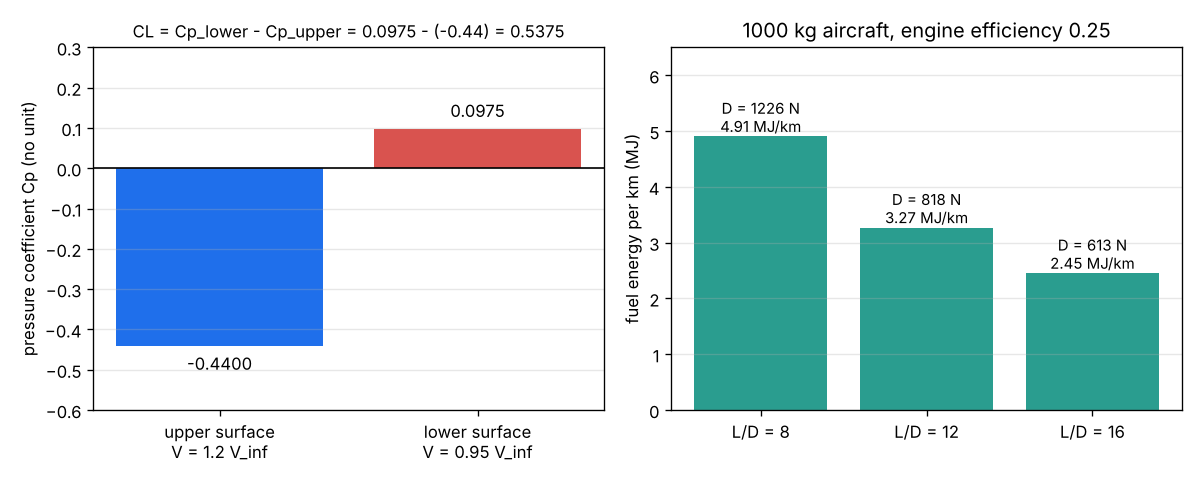
\includegraphics[width=0.85\linewidth]{figures/s01_pressure_and_fuel.png}\\\small Left: faster air on top gives suction and lift. Right: a better L/D cuts the fuel per kilometre.\end{center}

\subsection*{E. Worked example}
A 1000 kg aircraft with a 16 m2 wing cruises at 50 m/s at sea level. Find the dynamic pressure, the CL it needs and its stall speed for CL\_max = 1.4. With CD = 0.03, find the drag, L/D and the fuel energy per kilometre for an engine-and-propeller efficiency of 0.25. Finally find CL for a toy wing with air 1.2 times faster than V\_inf on top and 0.95 times underneath.
\begin{enumerate}[nosep]
\item q = 0.5 x 1.225 x 50\textasciicircum{}2 = 1531.25 Pa.
\item Weight = 1000 x 9.81 = 9810 N, so CL = 9810 / (1531.25 x 16) = 9810 / 24500 = 0.4004.
\item Stall speed = sqrt(2 x 9810 / (1.225 x 16 x 1.4)) = sqrt(19620 / 27.44) = sqrt(715.0) = 26.74 m/s.
\item Drag = 1531.25 x 16 x 0.03 = 735 N; L/D = 0.4004 / 0.03 = 13.35 (check: 9810 / 735 = 13.35).
\item Fuel energy per km = 735 N x 1000 m / 0.25 = 2.94 x 10\textasciicircum{}6 J = 2.94 MJ.
\item Toy wing: Cp\_upper = 1 - 1.2\textasciicircum{}2 = -0.44, Cp\_lower = 1 - 0.95\textasciicircum{}2 = 0.0975, CL = 0.0975 - (-0.44) = 0.5375.
\end{enumerate}
\textbf{Answer.} q = 1531 Pa, CL = 0.400, stall at 26.7 m/s; D = 735 N, L/D = 13.4, 2.94 MJ per km; toy wing CL = 0.54.

\subsection*{F. Questions}
\begin{enumerate}[nosep]
\item \textbf{Conceptual.} Why does a slow aircraft have to fly with its nose higher (a larger angle of attack) than a fast one, and why can it not fly slower than the stall speed?
\item \textbf{Numerical.} A wing of 12 m2 flies at 60 m/s at sea level with CL = 0.5. Find q and the lift. Can it hold up a 1200 kg aircraft? Check the units.
\item \textbf{Graph and simulation interpretation.} In the lift-against-speed figure, read the lift at CL = 0.6 at 40 m/s and at 80 m/s. By what factor does it grow, and why is the curve not a straight line?
\item \textbf{Design and optimisation challenge.} Design: choose the wing area of a 1000 kg aircraft so that it stalls at no more than 25 m/s with flaps giving CL\_max = 1.5. What CL will it then need in a 50 m/s cruise, and why would a designer not simply make the wing much bigger?
\end{enumerate}

\section{Session 2: Airfoil shape, thin-airfoil theory and the drag polar}

\subsection*{A. Real-world problem}
Session 1 found that our 1000 kg aircraft needs CL = 0.40 in cruise. Which wing section gives that, and at what angle? And once we know the lift, how large is the drag of the whole aircraft, and what is the best L/D it can reach? (Simplified low-speed model; not an aircraft design method.)

\subsection*{B. Concept and theory}
A wing section (airfoil) is described by its chord c (nose to tail), its camber line (the curved middle line) and its thickness wrapped round that line. The NACA 4-digit family names this with four digits: NACA 2412 has a maximum camber m = 2 percent of the chord at p = 4 tenths of the chord from the nose, and a maximum thickness of 12 percent. Thin-airfoil theory replaces the airfoil by its camber line covered with a sheet of tiny vortices, and demands that the air slides along the line and leaves the sharp trailing edge smoothly (the Kutta condition). The result is CL = 2 pi (alpha - alpha\_L0) with alpha in radians: the lift slope 2 pi per radian (0.110 per degree) is the same for every thin airfoil, and only the camber line sets the zero-lift angle alpha\_L0 through an integral of its slope. A symmetric airfoil has alpha\_L0 = 0; camber makes alpha\_L0 negative so the wing lifts even at zero angle; thickness does not appear at all. A real wing has a finite span b, and the air leaks round its tips. The tip vortices tilt the lift slightly backwards, which is an induced drag that grows with CL squared. With the aspect ratio AR = b\textasciicircum{}2 / S and a span efficiency e (about 0.7 to 0.9) the drag polar of the whole aircraft is CD = CD0 + CL\textasciicircum{}2 / (pi e AR), where CD0 is the parasite drag at zero lift (friction of the wing, fuselage, tail, wheels). L/D = CL / CD is largest where the two parts are equal, which gives CL* = sqrt(CD0 pi e AR) and (L/D)max = 1 / (2 sqrt(CD0 k)) with k = 1 / (pi e AR). Long, slender wings (gliders) have high AR and high L/D.

\begin{itemize}[nosep]
\item c: chord, nose to trailing edge (x and y are given as fractions of c) (m)
\item m, p, t: max camber, its position, max thickness (fractions of c) (no unit)
\item alpha: angle of attack between chord line and oncoming air (degrees or rad)
\item alpha\_L0: zero-lift angle of attack (degrees)
\item AR: aspect ratio b\textasciicircum{}2 / S (no unit)
\item e: span efficiency (1 for an ideal elliptical wing) (no unit)
\item CD0: parasite drag coefficient of the aircraft at zero lift (no unit)
\item k: induced-drag factor 1 / (pi e AR) (no unit)
\end{itemize}

\begin{equation*}
y_c = \frac{m}{p^2}\left(2 p x - x^2\right)\ (x<p),\qquad y_c = \frac{m}{(1-p)^2}\left(1 - 2p + 2 p x - x^2\right)\ (x\ge p)
\end{equation*}

\begin{equation*}
y_t = 5t\left(0.2969\sqrt{x} - 0.1260x - 0.3516x^2 + 0.2843x^3 - 0.1036x^4\right)
\end{equation*}

\begin{equation*}
C_L = 2\pi(\alpha - \alpha_{L0}),\qquad \alpha_{L0} = -\frac1\pi\int_0^\pi \frac{dy_c}{dx}\,(\cos\theta - 1)\,d\theta,\quad x = \tfrac12(1-\cos\theta)
\end{equation*}

\begin{equation*}
C_D = C_{D0} + k C_L^2,\qquad k = \frac{1}{\pi e A\!R},\qquad A\!R = \frac{b^2}{S}
\end{equation*}

\begin{equation*}
C_L^* = \sqrt{C_{D0}/k},\qquad (L/D)_{\max} = \frac{1}{2\sqrt{C_{D0}\,k}}
\end{equation*}

\begin{center}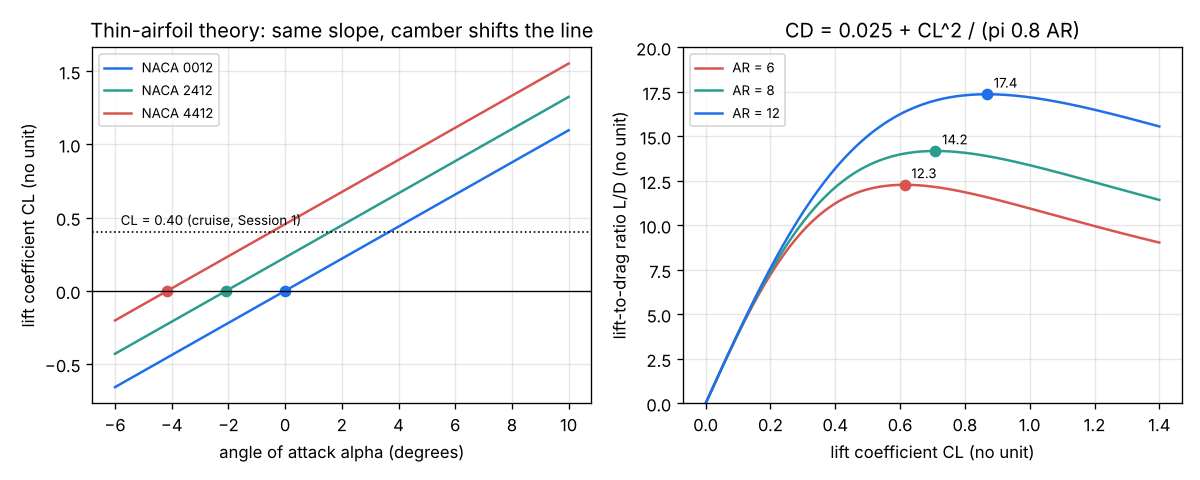
\includegraphics[width=0.85\linewidth]{figures/s02_lift_line_and_polar.png}\\\small Left: thin-airfoil lift lines, shifted by camber. Right: L/D of the drag polar for three aspect ratios.\end{center}

\subsection*{E. Worked example}
For NACA 2412 find m, p and t, the zero-lift angle, CL at 4 degrees and the angle needed for CL = 0.40 (thin-airfoil theory). The aircraft has AR = 8, e = 0.8 and CD0 = 0.025: find k, CD and L/D at CL = 0.40, and the best L/D.
\begin{enumerate}[nosep]
\item NACA 2412: m = 0.02, p = 0.4, t = 0.12.
\item The integral of the camber slope (computed in \texttt{alpha\_zero\_lift}) gives alpha\_L0 = -2.077 degrees, about -2.08.
\item CL(4 degrees) = 2 pi x (4 + 2.077) x pi / 180 = 6.283 x 0.10606 = 0.666.
\item Angle for CL 0.40: 0.40 / (2 pi) = 0.0637 rad = 3.65 degrees above alpha\_L0, so alpha = 3.65 - 2.08 = 1.57 degrees.
\item k = 1 / (pi x 0.8 x 8) = 1 / 20.11 = 0.04974. CD = 0.025 + 0.04974 x 0.16 = 0.025 + 0.00796 = 0.03296; L/D = 0.40 / 0.03296 = 12.1.
\item Best: CL* = sqrt(0.025 / 0.04974) = 0.709, (L/D)max = 1 / (2 sqrt(0.025 x 0.04974)) = 1 / (2 x 0.03526) = 14.2.
\end{enumerate}
\textbf{Answer.} alpha\_L0 = -2.08 degrees, CL(4 deg) = 0.666, alpha for CL 0.40 = 1.57 degrees; CD = 0.0330 and L/D = 12.1 at cruise; best L/D 14.2 at CL = 0.71.

\subsection*{F. Questions}
\begin{enumerate}[nosep]
\item \textbf{Conceptual.} Two airfoils have the same thickness but one is symmetric and one is cambered. According to thin-airfoil theory, how do their lift lines differ, and which one needs the smaller angle to give CL = 0.40?
\item \textbf{Numerical.} NACA 4412 has twice the camber of NACA 2412. Find its zero-lift angle and its CL at 2 degrees from thin-airfoil theory. Show the working.
\item \textbf{Graph and simulation interpretation.} In the L/D figure, how do the best L/D and the CL where it occurs change when the aspect ratio rises from 6 to 12? Explain the shape of each curve.
\item \textbf{Design and optimisation challenge.} Design: with CD0 = 0.025 and e = 0.8, what aspect ratio gives a best L/D of at least 15? For a 16 m2 wing, what span is that? Name two reasons not to choose a much larger AR.
\end{enumerate}

\section{Session 3: A panel method for lift, and an estimate of drag}

\subsection*{A. Real-world problem}
Thin-airfoil theory ignores thickness and gives no pressure along the surface, so it cannot tell us where the suction is or how the flow behaves near the nose. Can we compute the speed and pressure all round any airfoil, prove the code is right on a case with an exact answer, then estimate the airfoil's lift and drag and choose a wing section for our 1000 kg aircraft? (A simplified teaching model, not a design tool.)

\subsection*{B. Concept and theory}
We model low-speed air as a potential flow: steady, incompressible and frictionless. Such flows can be added together, so we build the flow round an airfoil from the free stream plus simple pieces. Cut the surface into N straight panels. Each panel j carries a source sheet of its own strength q\_j (air flows out of it) and a vortex sheet of one shared strength gamma (air swirls round it). The velocity a sheet induces at any point has a closed form in the panel's coordinates: a source gives u = q ln(r1 / r2) / (2 pi) and v = q beta / (2 pi), where r1 and r2 are the distances to the panel ends and beta is the angle the panel fills; a vortex gives the same pieces swapped. The N + 1 unknowns come from N + 1 equations: no flow through any panel at its midpoint (flow tangency) and the Kutta condition that the tangential speeds on the two panels at the trailing edge are equal in size. Solving the linear system gives the surface speed Vt, then Cp = 1 - Vt\textasciicircum{}2 (with V\_inf = 1), and summing the pressure times the panel length gives the force. A second, independent route is the Kutta-Joukowski theorem: the lift per unit span is rho V Gamma, so CL = 2 Gamma / (V c), with the circulation Gamma = gamma times the perimeter. The potential flow has no friction, so it predicts zero drag on any closed body (d'Alembert's paradox). Real airfoil drag at small angles is mostly skin friction in the thin boundary layer, which depends on the Reynolds number Re = V c / nu. A classic estimate uses the turbulent flat-plate law Cf = 0.074 / Re\textasciicircum{}0.2 on both surfaces, times a form factor for thickness: cd = 2 Cf (1 + 2 t/c + 60 (t/c)\textasciicircum{}4).

\begin{itemize}[nosep]
\item N: number of panels (160 in the lesson) (no unit)
\item q\_j: source strength of panel j (m/s (V\_inf = 1))
\item gamma, Gamma: vortex strength per length, total circulation (m/s, m2/s)
\item Vt: tangential surface speed relative to V\_inf (no unit)
\item Re: Reynolds number V c / nu (no unit)
\item nu: kinematic viscosity of air, 1.5e-5 (m2/s)
\item Cf: skin-friction coefficient of one surface (no unit)
\item cl, cd: section (2-D) lift and drag coefficients (no unit)
\end{itemize}

\begin{equation*}
\left(\vec V_\infty + \sum_j q_j \vec u^{\,s}_{ij} + \gamma \sum_j \vec u^{\,v}_{ij}\right)\cdot \hat n_i = 0,\quad i = 1..N
\end{equation*}

\begin{equation*}
V_{t,1} = -V_{t,N}\quad\text{(Kutta condition)}
\end{equation*}

\begin{equation*}
C_p = 1 - V_t^2,\qquad C_L = -\frac1c\sum_i C_{p,i}\,l_i\,(\hat n_i \times \hat e_{\infty})\quad\text{and}\quad C_L = \frac{2\Gamma}{c}
\end{equation*}

\begin{equation*}
Re = \frac{V c}{\nu},\qquad C_f = \frac{0.074}{Re^{0.2}},\qquad c_d = 2 C_f\left(1 + 2\frac tc + 60\left(\frac tc\right)^4\right)
\end{equation*}

\begin{center}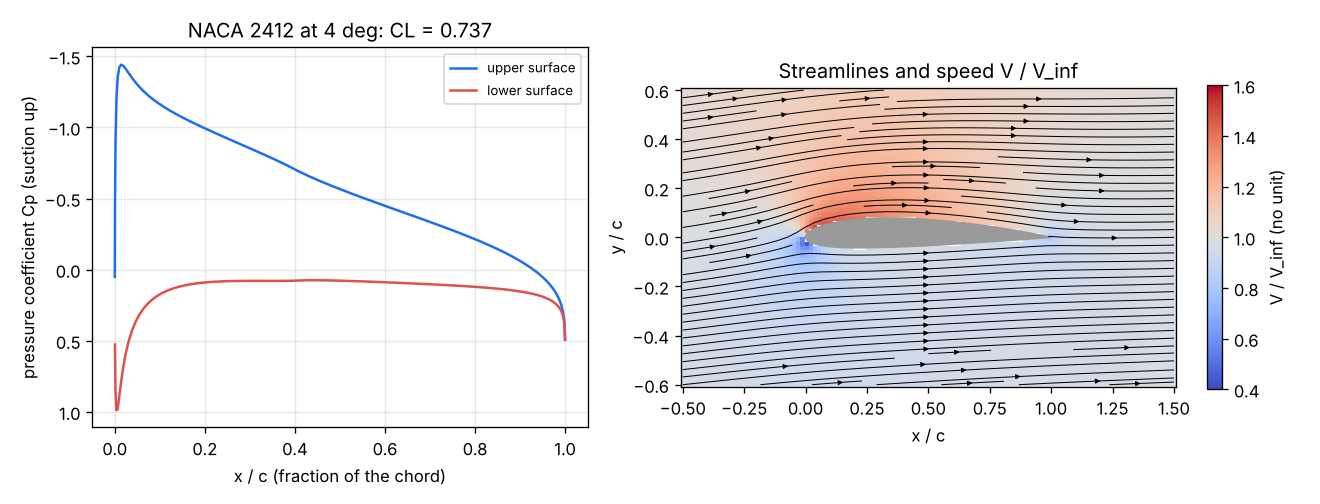
\includegraphics[width=0.85\linewidth]{figures/s03_pressure_streamlines.png}\\\small NACA 2412 at 4 degrees: surface pressure and streamlines from the panel method.\end{center}

\subsection*{E. Worked example}
Solve NACA 0012 at 5 degrees with 160 panels. Compare CL with thin-airfoil theory and with its thickness-corrected value 2 pi (1 + 0.77 t/c) alpha. Then estimate the drag for a 1.5 m chord at 50 m/s and the section L/D.
\begin{enumerate}[nosep]
\item Build the outline (80 points per side, cosine spacing) and solve the 161 x 161 system.
\item Panel results: CL from pressure = 0.6025, from circulation = 0.6052 (they agree within 0.5 percent); pressure drag 0.0002, nearly zero as d'Alembert says.
\item Thin-airfoil theory: 2 pi x 5 x pi / 180 = 0.548. Thickness-corrected: 0.548 x (1 + 0.77 x 0.12) = 0.599, within 0.6 percent of the panel value.
\item Re = 50 x 1.5 / 1.5e-5 = 5 x 10\textasciicircum{}6. Re\textasciicircum{}0.2 = 21.87, so Cf = 0.074 / 21.87 = 0.00338.
\item Form factor = 1 + 0.24 + 60 x 0.12\textasciicircum{}4 = 1.252; cd = 2 x 0.00338 x 1.252 = 0.00848.
\item Section L/D = 0.6025 / 0.00848 = 71.
\end{enumerate}
\textbf{Answer.} CL = 0.603 (thin theory 0.548, corrected 0.599), cd = 0.0085 at Re = 5 million, section L/D about 71.

\subsection*{F. Questions}
\begin{enumerate}[nosep]
\item \textbf{Conceptual.} The panel method gives almost zero drag on the airfoil. Is the code wrong? Where does the real drag come from?
\item \textbf{Numerical.} A model aircraft wing has a chord of 1.2 m and flies at 30 m/s. Find Re, Cf and the drag estimate cd for a 15 percent thick section.
\item \textbf{Graph and simulation interpretation.} In the pressure figure for NACA 2412 at 4 degrees, where is the lowest pressure, what is its Cp, and which surface contributes most of the lift?
\item \textbf{Design and optimisation challenge.} Design: the 1000 kg aircraft needs CL = 0.40 at 50 m/s (chord 1.5 m), a section at least 12 percent thick for the spar, and an angle of 0 to 3 degrees. Compare NACA 2408, 2412, 2415, 4412 and 0012 and choose one. What does the choice trade off?
\end{enumerate}

\section{Real-world mini-project}
\textbf{Choose the wing section of a small two-seater.} The 1000 kg aircraft of Session 1 cruises at 50 m/s with a 16 m2 wing of chord 1.5 m and needs CL = 0.40. The wing spar needs a section at least 12 percent thick, and the cabin floor should be level in cruise, so the wing must meet the air at 0 to 3 degrees. The candidates are NACA 2408, 2412, 2415, 4412 and 0012. Use \texttt{alpha\_for\_cl} and \texttt{cd\_profile} from Session 3 at Re = 5 million. These rules are illustrative, not a certification standard.

\section{The path ahead}
\begin{enumerate}[nosep]
\item \textbf{Session 4: A laminar boundary layer (Thwaites).} Thwaites' integral method marching along each surface from the stagnation point, using the panel Vt.
\item \textbf{Session 5: Transition and a turbulent boundary layer.} Michel's transition criterion and Head's entrainment method, with the drag from the Squire-Young formula at the trailing edge.
\item \textbf{Session 6: The drag polar of an airfoil.} cd from Session 5 for a sweep of angles, plotted as cl against cd, with the best section L/D marked.
\item \textbf{Session 7: Separation and an estimate of stall.} Detect separation from the shape factor H of the turbulent layer and reduce the effective lift as the separated part grows.
\item \textbf{Session 8: From airfoil to wing (Prandtl lifting line).} A lifting-line solver with a Fourier series for the circulation along the span, fed with the section lift slope from Session 3.
\end{enumerate}

\section{Answers and hints}

\subsection*{Session 1}
\begin{enumerate}[nosep]
\item \textbf{Conceptual.} Hint: Look at CL = m g / (q S) and remember q grows with V squared. Solution: The weight is fixed, so q S CL must stay equal to m g. When V halves, q falls to a quarter, so CL must grow four times. The wing gets more CL by meeting the air at a larger angle. But CL cannot grow forever: above CL\_max the air separates from the upper surface and the lift drops (stall). The speed at which the needed CL equals CL\_max is the stall speed; slower than that the wing cannot hold up the weight.
\item \textbf{Numerical.} Hint: q = 1/2 rho V\textasciicircum{}2, then L = q S CL; compare with m g. Solution: q = 0.5 x 1.225 x 3600 = 2205 Pa. L = 2205 x 12 x 0.5 = 13230 N = 13.2 kN. Weight = 1200 x 9.81 = 11772 N. Since 13.2 kN is more than 11.8 kN, yes (it would climb, or it can fly at a smaller CL). Units: Pa x m2 = N.
\item \textbf{Graph and simulation interpretation.} Hint: Lift is proportional to V squared. Solution: About 9.4 kN at 40 m/s and 37.6 kN at 80 m/s: a factor of 4 for twice the speed, because q = 1/2 rho V\textasciicircum{}2 grows with the square of V. A straight line would mean lift proportional to V, which is wrong.
\item \textbf{Design and optimisation challenge.} Hint: Solve the stall-speed formula for S: S = 2 m g / (rho V\textasciicircum{}2 CL\_max). Solution: S = 2 x 9810 / (1.225 x 625 x 1.5) = 19620 / 1148.4 = 17.1 m2. In cruise q = 1531 Pa, so CL = 9810 / (1531 x 17.1) = 0.375. Trade-off: a bigger wing lands slower but has more surface rubbing against the air (more friction drag in cruise), more weight and more cost; designers use flaps to raise CL\_max for landing instead of carrying a huge wing all the time.
\end{enumerate}

\subsection*{Session 2}
\begin{enumerate}[nosep]
\item \textbf{Conceptual.} Hint: Which quantity in CL = 2 pi (alpha - alpha\_L0) depends on camber? Solution: The slope 2 pi per radian is the same for both; only the zero-lift angle differs. The cambered airfoil has a negative alpha\_L0, so its line is shifted left and it gives the same CL at a smaller angle (for NACA 2412, 1.57 degrees against 3.65 for NACA 0012).
\item \textbf{Numerical.} Hint: Thin-airfoil alpha\_L0 is proportional to m for a fixed p. Solution: alpha\_L0 = 2 x (-2.077) = -4.15 degrees. CL = 2 pi x (2 + 4.154) x pi / 180 = 6.283 x 0.1074 = 0.675. Sanity check: it is between 0 and the stall value of about 1.5, and above the NACA 2412 value at 2 degrees (0.447).
\item \textbf{Graph and simulation interpretation.} Hint: Read the dots; the left side is dominated by CD0, the right side by induced drag. Solution: Best L/D rises from 12.3 (at CL 0.61) to 17.4 (at CL 0.87). At small CL the drag is mostly CD0, so L/D grows almost in proportion to CL; at large CL the induced drag k CL\textasciicircum{}2 dominates and L/D falls like 1 / (k CL). A higher AR shrinks k, so the induced part matters later and the peak is higher and further right.
\item \textbf{Design and optimisation challenge.} Hint: Invert (L/D)max = 0.5 sqrt(pi e AR / CD0): AR = 4 (L/D)\textasciicircum{}2 CD0 / (pi e). Solution: AR = 4 x 225 x 0.025 / (pi x 0.8) = 22.5 / 2.513 = 8.95, so about 9 (best L/D 15.0). Span b = sqrt(AR S) = sqrt(9 x 16) = 12 m. Trade-offs: a long, slender wing must be stronger and so heavier at the root (larger bending moment), it needs a bigger hangar and parking space, and it rolls more slowly. Gliders accept these for L/D of 40 or more.
\end{enumerate}

\subsection*{Session 3}
\begin{enumerate}[nosep]
\item \textbf{Conceptual.} Hint: Think about which physical effect the potential-flow model leaves out. Solution: The code is right: an inviscid, steady flow round a closed body in two dimensions has zero drag (d'Alembert's paradox), and the small leftover 0.0002 is numerical error that shrinks with more panels. Real airfoil drag comes from viscosity: skin friction in the boundary layer and, at larger angles, pressure drag from a thick or separated wake. That is why we add the friction estimate separately.
\item \textbf{Numerical.} Hint: Re = V c / nu with nu = 1.5e-5; then Cf = 0.074 / Re\textasciicircum{}0.2 and the form factor. Solution: Re = 30 x 1.2 / 1.5e-5 = 2.4 x 10\textasciicircum{}6. Re\textasciicircum{}0.2 = 18.88, Cf = 0.074 / 18.88 = 0.00392. Form factor = 1 + 0.30 + 60 x 0.15\textasciicircum{}4 = 1.330. cd = 2 x 0.00392 x 1.330 = 0.0104. It is larger than the 0.0085 of the worked example because Re is lower (more friction) and the section is thicker.
\item \textbf{Graph and simulation interpretation.} Hint: The Cp axis is drawn upside down so suction points up; lift is the area between the curves. Solution: The suction peak is on the upper surface very close to the nose (x/c about 0.01), with Cp about -1.44. The upper curve encloses most of the area: the lower surface has a small positive Cp of about +0.1. So most of the lift is suction on the top, not push on the bottom. The peak is also where the boundary layer is most at risk later: after it the pressure rises towards the trailing edge.
\item \textbf{Design and optimisation challenge.} Hint: Use \texttt{choose\_section} from the lesson. Solution: Angles for CL 0.40: 2408 1.34, 2412 1.20, 2415 1.10, 4412 -0.91 and 0012 3.32 degrees. Drag estimates: 0.00787, 0.00848, 0.00900, 0.00848 and 0.00848. NACA 2408 has the lowest drag but is too thin; 4412 needs a negative angle and 0012 more than 3 degrees. NACA 2412 meets every rule with the lowest drag (section L/D about 47) and is chosen. Trade-off: a thicker section is stronger and lighter to build but has more drag; the angle rule is about the cabin attitude, not aerodynamics. The friction estimate does not see camber, so a real comparison needs the boundary-layer model of the roadmap.
\end{enumerate}

\section{Further reading}
\begin{itemize}[nosep]
\item I. H. Abbott and A. E. von Doenhoff, \emph{Theory of Wing Sections}, Dover, 1959 (NACA airfoils and wind-tunnel data).
\item J. Katz and A. Plotkin, \emph{Low-Speed Aerodynamics}, 2nd ed., Cambridge University Press, 2001 (panel methods).
\item J. D. Anderson, \emph{Fundamentals of Aerodynamics}, McGraw-Hill (thin-airfoil theory, drag polar).
\end{itemize}

\section{How to join}
Read \texttt{CONTRIBUTING.md} in the repository, then pick an issue labelled \texttt{good first issue}. Repository: \url{https://github.com/KrunalPanchal1995/pan-iit-oss/tree/main/openairfoil}

\end{document}
